%% Cheat-Sheet for our SSY-LB repo

% to include a Matlab-Src
\lstinputlisting{path}

% to include a picture
\begin{figure}[htbp]				% set the position of the whole figure
\centering
\includegraphics[scale=0.2]{path}	% set the path for the pic. scale to fit to page
\caption{Text}						% set a descriptive Text
\label{fig:key}						% Keyword to refer to this figure
\end{figure}

% to create a table
\begin{table}[h]
\begin{tabular}{c | c | c}					% the table per se, {alignment of the columns(rcl) '|' vertical line}]
Funktionsblock & Parameter & Wert\\
\hline										% horizontal line
Sine Wave & Sine type & Time based \\
& Time (t) & Use simulation time \\			% '&' to move to next cell
& Amplitude & 0.5\\							% '\\' to end this row

\end{tabular}
\caption{Text}								% set a descriptive Text
\label{tab:ref}								% Keyword to refer to this table
\end{table}



% to draw a diagram - not a lot of experience with it
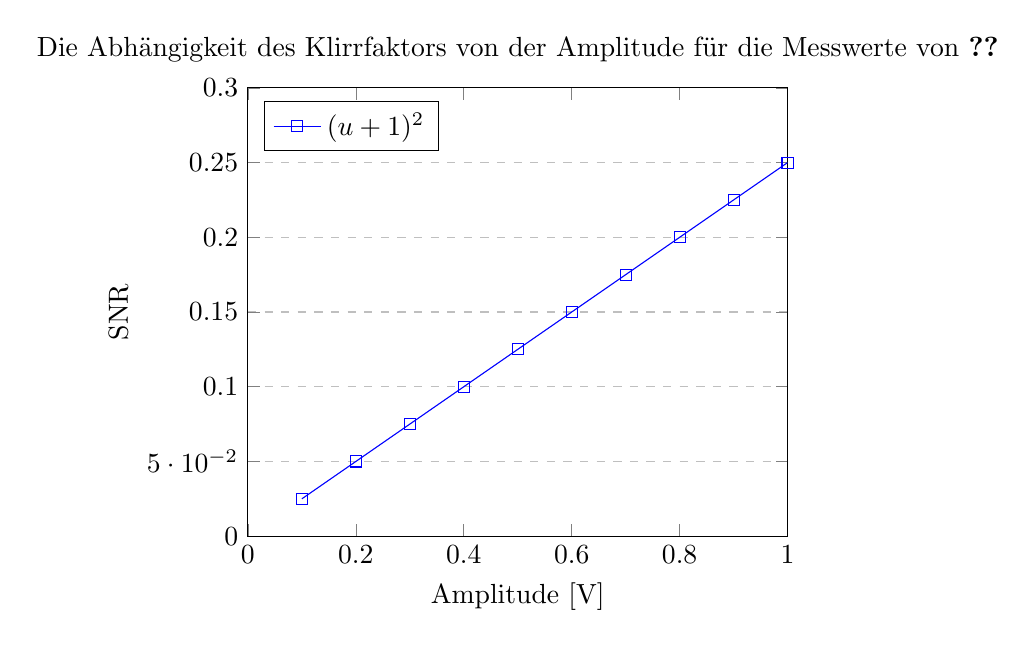
\begin{tikzpicture}
\centering
\begin{axis}[
    title={Die Abhängigkeit des Klirrfaktors von der Amplitude für die Messwerte von \ref{tab:messw_klirr}},
    xlabel={Amplitude [V]},
    ylabel={SNR},
    xmin=0, xmax=1.0,
    ymin=0, ymax=0.3,
    xtick={0,0.2,0.4,.6,.8,1.0},
    ytick={0,0.05, 0.1, 0.15, 0.20, 0.25, 0.3},
    legend pos=north west,
    ymajorgrids=true,
    grid style=dashed,
]
 
\addplot[
    color=blue,
    mark=square,
    ]
    coordinates {
    (0.1,0.02501)(0.20,0.05)(0.30,0.075)(0.40,0.1)(0.5, 0.125)(0.60,0.15)(0.7, 0.175)(0.80, 0.2)(0.9, 0.225)(1.00,0.25)
    };
    \legend{$(u+1)^2$}
 
\end{axis}

\end{tikzpicture}


% to create a reference to a text
Im Vergleich von Abbildung \ref{fig:eing} zu \ref{fig:verr} kann man sehen, dass Oberwellen hinzugekommen sind.

% to create a complex equation
\begin{equation}
y(x) = \left\{
  \begin{array}{l l}
    \frac{1+ln(A*x)}{1+ln(A)} & \quad \text{$\frac{1}{A} \le x \le 1$}\\
    \frac{A*x}{1+ln(A)} & \quad \text{$-\frac{1}{A} \le x \le \frac{1}{A}$}\\
    -\frac{1+ln(-A*x)}{1+ln(A)} & \quad \text{$-1 \le x \le -\frac{1}{A}$}
  \end{array} \right.
\end{equation}